Consider the Atwood's machine shown in Fig.~1.7, consisting of three masses and three frictionless pulleys. It can be shown that the acceleration of $m_1$ is given by (just accept this): $$a_1 = g \frac{3m_2 m_3 - m_1(4m_3 + m_2)}{m_2 m_3 + m_1(4m_3 + m_2)}, \tag{1.18}$$ with upward taken to be positive. Find $a_1$ in the following special cases:

\begin{enumerate}
\item $m_2 = 2m_1 = 2m_3$.
\item $m_1$ much larger than both $m_2$ and $m_3$.
\item $m_1$ much smaller than both $m_2$ and $m_3$.
\item $m_2 \gg m_1 = m_3$.
\item $m_1 = m_2 = m_3$.
\end{enumerate}

\begin{center}
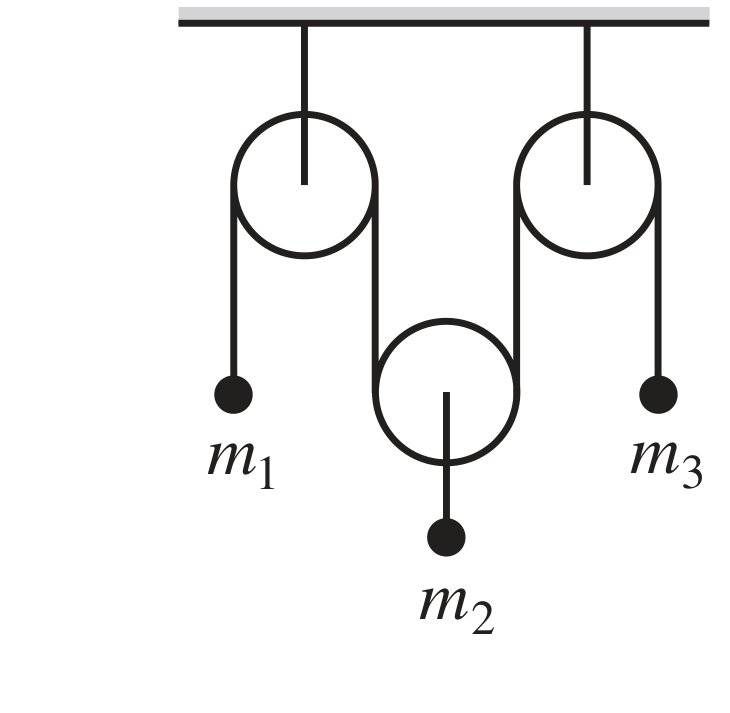
\includegraphics[width=0.35\linewidth]{figures/qfig1.png} \\ Fig.~1.7
\end{center}